% !TeX spellcheck = en_US
\documentclass[letterpaper,12pt,twoside]{report}
\usepackage{fancyhdr}
\usepackage{fullpage}
\usepackage{tikz}
\usepackage{amsmath}

\begin{document}
	\pagestyle{fancy}
	\fancyhf{}
	\fancyhead[L]{Day 27}
	\fancyhead[R]{\textit{The Calendar Project}}
	\fancyfoot[L]{Citations Involved: none}
	
	% Problem
	\paragraph{Problem}
	\begin{quote}
		\textsf{Two circles “fit” perfectly in a $2 \times 1$ rectangle because each can be inscribed in a $1 \times 1$ square. What fraction of the rectangle's area lies within the two circles?}
	\end{quote}
	
	% Graphics
	\begin{center}
		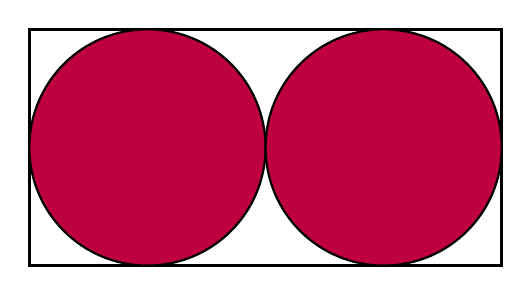
\begin{tikzpicture}[scale=3]
		\draw[very thick] (-1,1) -- (1,1) -- (1,0) -- (-1,0) -- cycle;
		\draw[thick][fill=purple] (-0.5,0.5) circle [radius=0.5];
		\draw[thick][fill=purple] (0.5,0.5) circle [radius=0.5];
		\end{tikzpicture}
	\end{center}
	
	% Reasoning
	\paragraph{Reasoning}
	\begin{quotation}
		
		Given that each circle is inscribed in a $1 \times 1$ square, they have a diameter of $1$ and therefore a radius of $\frac{d}{2}=\frac{1}{2}$. Using the circle area formula $r^2\pi$ (2), it is determined that both circles have an area of $(\frac{1}{2})^2\pi=\frac{\pi}{4}$. The total area of two such circles is $2(\frac{\pi}{4})=\frac{\pi}{2} \textrm{unit}^2$. The $2 \times 1$ rectangle has an area of $2 \times 1=2 \textrm{unit}^2$ (1). The fraction of the rectangle's area that lies within the two circles is $\frac{\frac{\pi}{2}}{2}=\pi \div 2 \div 2=\boxed{\frac{\pi}{4}}$. 
		
	\end{quotation}
	
	\paragraph{External References}
	
	\begin{enumerate}
		\item Textbook Ch. 9, Pg. 589: Area of a Parallelogram
		\item Textbook Ch. 9, Pg. 600: Circumference and Area of a Circle
	\end{enumerate}
	
\end{document}